\documentclass[conference,compsoc,final,a4paper]{IEEEtran}
\usepackage[utf8]{inputenx}

%% Bitte legen Sie hier den Titel und den Autor der Arbeit fest
\newcommand{\autorA}[0]{Büchner, Jannis}
\newcommand{\autorB}[0]{Büchner, Niklas}
\newcommand{\autorC}[0]{Vierling, Jörg}
\newcommand{\dokumententitel}[0]{Tik-Tak-Toe Roboter}

% Hie muss normalerweise nichts angepasst werden
\usepackage[pdftex]{graphicx}
\graphicspath{{img/}}
\DeclareGraphicsExtensions{.pdf,.jpeg,.jpg,.png}
\usepackage[cmex10]{amsmath}
\usepackage{algorithmic}
\usepackage{array}
\usepackage{dblfloatfix}
\usepackage{url}
\usepackage[autostyle=true,german=quotes]{csquotes}
\usepackage[backend=biber,
            sorting=none,   % Keine Sortierung
            doi=true,       % DOI anzeigen
            isbn=false,     % ISBN nicht anzeigen
            url=true,       % URLs anzeigen
            maxnames=6,     % Ab 6 Autoren et al. verwenden
            minnames=1,     % und nur den ersten Autor angeben
            style=ieee,]{biblatex}
\usepackage{booktabs}
\usepackage{xcolor}
\usepackage{listings}             % Source Code listings
\usepackage[printonlyused]{acronym}
\usepackage{fancyvrb}
\usepackage{tocloft} % Schönere Inhaltsverzeichnisse
\usepackage{amsmath}
\usepackage{siunitx}
\usepackage{booktabs}


% Farben definieren
\definecolor{linkblue}{RGB}{0, 0, 100}
\definecolor{linkblack}{RGB}{0, 0, 0}
\definecolor{darkgreen}{RGB}{14, 144, 102}
\definecolor{darkblue}{RGB}{0,0,168}
\definecolor{darkred}{RGB}{128,0,0}
\definecolor{comment}{RGB}{63, 127, 95}
\definecolor{javadoccomment}{RGB}{63, 95, 191}
\definecolor{keyword}{RGB}{108, 0, 67}
\definecolor{type}{RGB}{0, 0, 0}
\definecolor{method}{RGB}{0, 0, 0}
\definecolor{variable}{RGB}{0, 0, 0}
\definecolor{literal}{RGB}{31,0, 255}
\definecolor{operator}{RGB}{0, 0, 0}

\usepackage[ngerman]{betababel}

\DefineBibliographyStrings{ngerman}{
    andothers = {{et al\adddot}},  % Immer et al. sagen, auch bei Deutsch als Sprache
}
\usepackage[
      unicode=true,
      hypertexnames=false,
      colorlinks=true,
      colorlinks=false,
      linkcolor=darkblue,
      citecolor=darkblue,
      urlcolor=darkblue,
      pdftex
   ]{hyperref}
%	 \PrerenderUnicode{ü}


% Einstellungen für Quelltexte
\lstset{
    xleftmargin=0.1cm,
    basicstyle=\scriptsize\ttfamily,
    keywordstyle=\color{keyword},
    identifierstyle=\color{variable},
    commentstyle=\color{comment},
    stringstyle=\color{literal},
    tabsize=2,
    lineskip={2pt},
    columns=flexible,
    inputencoding=utf8,
    captionpos=b,
    breakautoindent=true,
    breakindent=2em,
    breaklines=true,
    prebreak=,
    postbreak=,
    numbers=none,
    numberstyle=\tiny,
    showspaces=false,      % Keine Leerzeichensymbole
    showtabs=false,        % Keine Tabsymbole
    showstringspaces=false,% Leerzeichen in Strings
    morecomment=[s][\color{javadoccomment}]{/**}{*/},
    literate={Ö}{{\"O}}1 {Ä}{{\"A}}1 {Ü}{{\"U}}1 {ß}{{\ss}}2 {ü}{{\"u}}1 {ä}{{\"a}}1 {ö}{{\"o}}1
}

\hypersetup{
    pdftitle={\dokumententitel},
    pdfauthor={\autoren},
    pdfdisplaydoctitle=true,
    hidelinks
}

% Makros für typographisch korrekte Abkürzungen
\newcommand{\zb}[0]{z.\,B.\ }
\newcommand{\dahe}[0]{d.\,h.\ }
\newcommand{\ua}[0]{u.\,a.\ }

% Wo liegt Sourcecode?
\newcommand{\srcloc}{src/}

% Literatur einbinden
\addbibresource{literatur.bib}
 % Weitere Einstellungen aus einer anderen Datei lesen

\begin{document}

% Titel des Dokuments
\title{\dokumententitel}

% Namen der Autoren
\author{
  \IEEEauthorblockN{
    \autorA\\
    \autorB\\
    \autorC
  }
  \IEEEauthorblockA{
    Hochschule Mannheim\\
    Fakultät für Informatik\\
    Paul-Wittsack-Str. 10,
    68163 Mannheim
    }
}

% Titel erzeugen
\maketitle
\thispagestyle{plain}
\pagestyle{plain}

% Eigentliches Dokument beginnt hier
% ----------------------------------------------------------------------------------------------------------

% Kurze Zusammenfassung des Dokuments
\begin{abstract}

Im Rahmen der Veranstaltung autonome mobile Roboter wird das Ziel verfolgt einen Roboter zu konstruieren, der in der Lage ist, auf einem Blatt Papier Tik-Tak-Toe zu spielen. Dieser Bericht beschreibt, wie die Mechanik, Elektronik und die Software erstellt wurden. 
Die Herausforderung besteht vor allem darin, die Schnittstellen zwischen den einzelnen Komponenten zu realisieren. Die Mechanik basiert auf Fischertechnik und ermöglicht den Bau eines Plotters, der Bewegungen in alle drei Raumrichtungen unabhängig voneinander erlaubt. Währenddessen besteht die Elektronik aus den Bauteilen des Roboter Kits von Freenove mit dem ESP32-WROVER. Damit die Motoren an das Breadboard von Freenove angeschlossen werden können, müssen bestehende Kabel von beiden Systemen mithilfe von Stoßverbinder fest verbunden werden. Dabei trat zum einen das Problem auf, dass das Board nur maximal \qty{5}{V} Versorgungsspannung liefern kann, während die Motoren \qty{9}{V} benötigen. Zum anderen muss eine Lösung gefunden werden, die Motoren in beide Richtungen drehen zu lassen. Beide Probleme können gelöst werden indem drei Motortreiber, vom Typ L293D,  genutzt werden. Diese erlauben zum einen die Bestimmung der Drehrichtung und zum anderen kann so ein separater Stromkreis aufgebaut werden, der die geforderten \qty{9}{V} an die Motoren liefert. Als nächstes muss die Kommunikation mit dem Nutzer realisiert werden. Dies gelingt über ein Keypad. Jedem der neun möglichen Feldern beim Tik-Tak-Toe ist eine Zahl zwischen eins und neun zugeordnet. Durch das Drücken der entsprechenden Taste fährt der Roboter in die gewünschte Position. Der Algorithmus selbst ist in C implementiert und auf den ESP32-WROOM eingebettet. 
Das Endergebnis des Projekts ist ein ein Plotter, der gegen einen Nutzer Tik-Tak-Toe spielen kann. Der Roboter mahlt zu Beginn des Spiels das Feld, wählt selbst das beste Feld aus um sein Zeichen zu setzen und erkennt am Ende ob ein Spieler gewonnen hat.

\end{abstract}

% Inhaltsverzeichnis erzeugen
{\small\tableofcontents}

\section{Projektziel}

Ziel dieses Projektes war es einen kleinen Roboter zu entwickeln, der Tik-Tak-Toe
auf einem Blatt Papier gegen den Nutzer spielen kann. Hierbei wurde Tik-Tak-Toe
gewählt, da es ein simples aber sehr bekanntes Spiel ist.

Das Team hat sich gegen die Nutzung eines schon existierenden Roboters oder Roboter-Kit
entschieden, um mit allen Bereichen der Robotik in Kontakt zu kommen. Ziel war es hier
eine Fachschafts übergreifende Kooperation zu nutzen, um einen optimalen Wissenstransfer
zu erreichen.

Um das Spiel Tik-Tak-Toe spielen zu können soll der Roboter in der Lage sein das Spielfeld
sowie die Züge aller Spieler zu zeichnen. 

Daraus ergab sich die grundsätzlichen Anforderung
an die Hardware, dass sie eine Bewegung in alle drei Raumrichtungen unabhängig voneinander
ermöglichen muss. Zudem sollte diese robust gestaltet und einfach zu realisieren sein.
Deswegen wurde entschieden einen Plotter zu bauen anstelle eines komplizierteren
Roboterarms. Dies hatte vor allem den Vorteil, dass die Bewegungen einfach zu realisieren
sind, ohne komplizierte Koordinatentransformationen durchführen zu müssen.


\section{Mechanik}

Da zu Beginn des Projekts kein Roboter vorhanden war, musste nicht nur der Code geschrieben, sondern auch die Hardware
konstruiert werden. Die grundsätzlichen Anforderungen an die Hardware waren, dass sie eine Bewegung in alle drei Raumrichtungen
unabhängig voneinander ermöglichen muss, robust gestaltet und einfach zu realisieren sein sollte. Deswegen wurde entschieden einen
Plotter zu bauen anstelle eines komplizierteren Roboterarms. Dies hat vor allem den Vorteil, dass die Bewegungen einfach zu
realisieren sind, ohne komplizierte Koordinatentransformationen durchführen zu müssen. In diesem Kapitel wird die mechanische Konstruktion
vorgestellt. Hierbei wird zuerst auf allgemeine Aspekte des Aufbaus eingegangen und anschließend die Bewegung in die einzelnen Achsen erläutert.

\subsection{Allgemeiner Aufbau}

Um den Plotter zu bauen wird Fischertechnik eingesetzt. Zum einen waren davon schon Teile vorhanden, zum anderen erfüllen diese
Materialien die Anforderungen an Robustheit ausreichend. Des Weiteren lassen sich lineare Bewegungen mithilfe von Spindelgetrieben
 einfach realisieren.

Die Spindelgetriebe haben den Vorteil, dass sie aus einzelnen Schneckenteilen bestehen, die nacheinander auf eine Achse geschoben
werden und dadurch in verschiedenen Längen konstruiert werden können. Damit die Schneckenteile nicht verrutschen, befinden sich an
den Enden klemmbare Schnecken, die mithilfe von Spannzangen fixiert werden. Letztlich befindet sich an jeder Achse noch ein Zahnrad,
das zum Antrieb des Spindelgetriebes genutzt wird.

Die Bewegungen in $x$, $y$ und $z$-Richtung werden separat voneinander gesteuert. Im Prinzip ist der Plotter somit aus drei Schichten
aufgebaut. Die unterste Schicht, der Grundrahmen, ist für die Bewegung in $x$-Richtung, also vor und zurück, zuständig. Darauf
sitzen zwei $y$-Schlitten, die die mittlere Schicht darstellen. Diese sorgt für die Bewegung nach links und rechts, in $y$-Richtung.
Darauf sitzt der Stiftehalter, der in $z$-Richtung nach oben und unten bewegt werden kann.

Der Grundrahmen besteht aus jeweils einer Achse und einem Spindelgetriebe, die sich links und rechts am Plotter befinden und an
den Enden auf zwei Basisplatten befestigt sind. Auf jedem Paar aus Achse und Spindelgetriebe befindet sich ein $y$-Schlitten, welcher
durch die Drehbewegung des Spindelgetriebes nach vorne und hinten bewegt wird. Die Aufgabe der Achsen ist, die Lasten und Momente
aufzunehmen. Aus diesem Grund müssen auch zwei Achsen verbaut werden, eine reicht nicht aus.
Theoretisch wäre es möglich gewesen, nur ein Spindelgetriebe einzubauen. Das hätte aber andere Probleme mit sich gebracht. Wären beide Achsen auf derselben Seite des Plotters angebracht worden, wäre das zu kompensierende Drehmoment sehr groß. Die andere Option, die Achsen auf gegenüberliegende Seiten des Plotters anzubringen, hätte bedeutet, dass sich die beiden Schlitten nicht gleichmäßig bewegen, sondern verzerrt bewegt hätten.

\subsection{$x$-Achse}

Damit sich die Spindelgetriebe der $x$-Achse gleich schnell und gleichzeitig drehen, sind diese mithilfe von einer Kette (bestehend aus einzelnen
Rastkettengliedern) verbunden. Dadurch wird eine gleichmäßige Bewegung gewährleistet und die Schlitten, die obendrauf sitzen,
verziehen sich nicht. Die Bewegung in x-Richtung wird durch einen XM-Motor von Fischertechnik ausgeführt, welcher auf einer
Basisplatte sitzt und eines der Getriebe mithilfe von Zahnrädern antreibt. Der Aufbau des Antriebes der $x$-Achse ist in Abbildung \ref{fig:AufbauxAchse} zu sehen.


\begin{figure}[h]
\centering
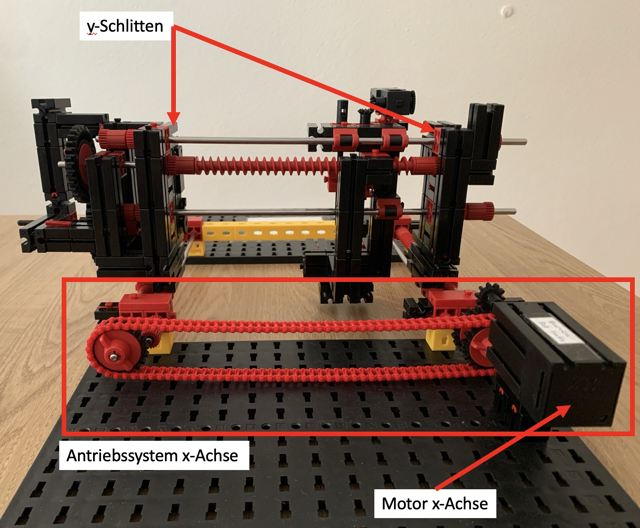
\includegraphics[width=8cm]{../images/xAchse1.png}
\caption{Antriebssystem der $x$-Achse (Ansicht von hinten)}
\label{fig:AufbauxAchse}
\end{figure}

\subsection{$y$-Achse}

Die zwei y-Schlitten sind ebenfalls mit zwei Achsen und einem Spindelgetriebe verbunden. Auch hier nehmen die Achsen das Gewicht
sowie das resultierende Drehmoment des Stiftehalter auf. Im Gegensatz zum Aufbau in $x$-Richtung befinden sind diese übereinander angeordnet,
damit der Aufbau nicht zu sehr nach vorne ragt, sondern stattdessen in die Höhe. Dadurch, dass die Achsen übereinander liegen, wirkt ein Moment auch auf die Schlitten an sich. Wenn der Stift also zu stark auf das Papier gedrückt wird, wird der Aufbau etwas nach hinten gedrückt. Dieses Problem wäre nicht vorhanden, wenn die Achsen nebeneinander angeordnet wären. Dafür würde der Aufbau in das Sichtfeld des Nutzers ragen und die Bewegung in $x$-Richtung wäre weiter eingeschränkt. 
Der Motor (Motor XS von Fischertechnik), der die y-Bewegung ausführt, ist etwas leistungsschwacher als der für die $x$-Bewegung. Dies hat
den Vorteil, dass er sehr viel kleiner und leichter ist. Dadurch kann er direkt auf einem der zwei y-Schlitten angebracht werden (Siehe Abbildung \ref{fig:AufbauyAchse1}). 

\begin{figure}[h]
\centering
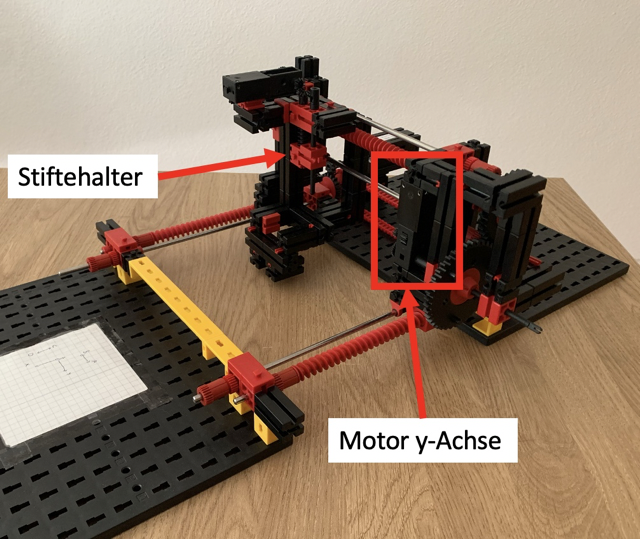
\includegraphics[width=8cm]{../images/yAchse1.png}
\caption{Motor, der am linken $y$-Schlitten angebracht ist und Stiftehalter}
\label{fig:AufbauyAchse1}
\end{figure}

Auch hier wird die Kraftübertragung zwischen der Antriebswelle des Motors und der Abtriebswelle des
Spindelgetriebes mithilfe von Zahnrädern ermöglicht. Das gesamte Antriebssystem der $y$-Achse ist in Abbildung \ref{fig:AufbauyAchse2} dargestellt.

\begin{figure}[h]
\centering
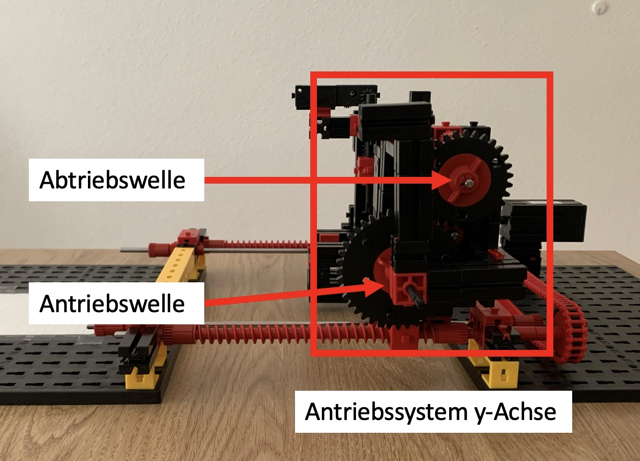
\includegraphics[width=8cm]{../images/yAchse2.png}
\caption{Antriebssystem der $y$-Achse bestehend aus dem Abtriebsrad und Antriebsrad (Ansicht von der Seite)}
\label{fig:AufbauyAchse2}
\end{figure}

\subsection{$z$-Achse}

Auf der $y$-Achse befindet sich ein weiterer Schlitten, welcher die $z$-Achse darstellt und der im Großen und Ganzen aus zwei Teilen besteht. 
Der eine Teil ist für das Anheben und Absetzen des Stiftes zuständig. Dieser besteht aus einer Rastachse mit Schnecke, die über
Kegelzahnräder bewegt wird. Auf der Schnecke befindet sich eine Schneckenmutter, an der ein regulärer Baustein 15 mit Bohrung angebracht ist. Durch die Bohrung verläuft eine Achse. Bei Drehung der Rastwelle bewegen sich die Schneckenmutter und das Bauteil gemeinsam nach oben oder unten. In Abbildung ... ist die Schneckenmutter mitsamt der Rastwelle und dem Baustein 15 dargestellt.
An diesem Mechanismus befindet sich der Stiftehalter. Das Ziel bei der Konstruktion des Stiftehalters war, ein einfacher, effizienter und
effektiver Aufbau, mit dem der Stift sowohl angehoben als auch mit Druck abgesetzt werden kann. Des Weiteren sollte es möglich sein, viele
verschiedenen Arten von Stifte zum Spielen verwenden zu können. Die beste Lösung für dieses Problem war den Stift mithilfe von Tesa-Film
an zwei Bausteine zu kleben, wie es in Abbildung \ref{fig:AufbauzAchse1} zu sehen ist. 

\begin{figure}[h]
\centering
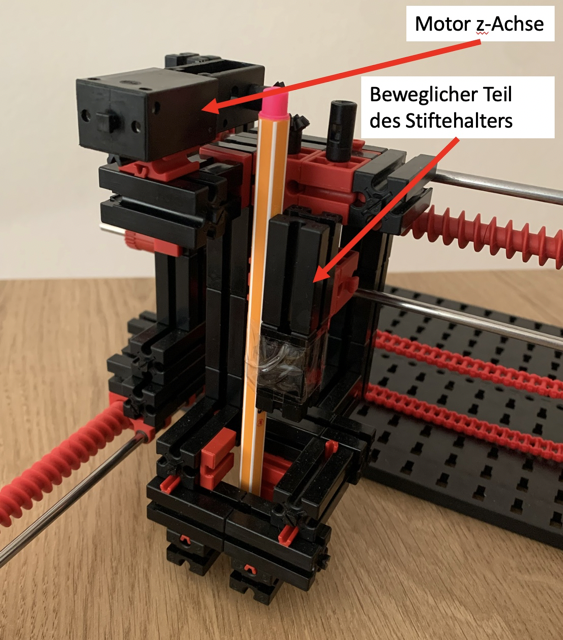
\includegraphics[width=8cm]{../images/zAchse1.png}
\caption{An Stiftehalter angeklebter Stift. }
\label{fig:AufbauzAchse1}
\end{figure}

\begin{figure}[h]
\centering
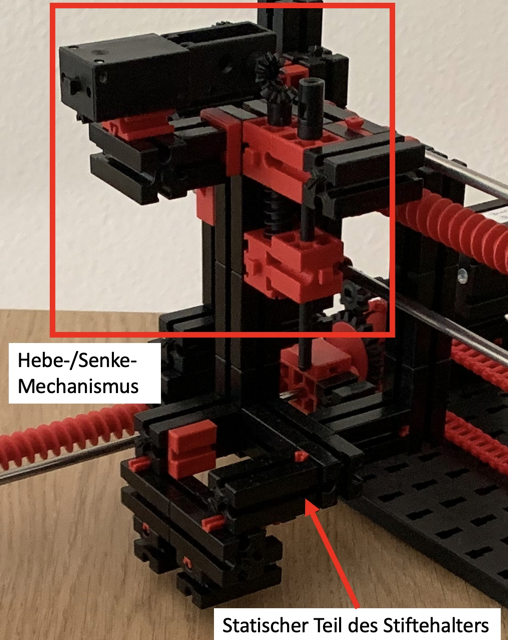
\includegraphics[width=8cm]{../images/zAchse2.png}
\caption{Stifthalter ohne angeklebter Stift. Im roten Kasten ist der bewegliche Teil des Stiftehalters zu sehen. Wenn sich der Motor dreht bewegen sich die zwei roten Bausteine, die 
sich unten im Kasten befinden, hoch und runter. Der restliche Teil der Konstruktion ist starr und soll ein Verbiegen und Verzerren des Stiftes und Hebemechanismus verhindern.}
\label{fig:AufbauzAchse2}
\end{figure}

Der zweite Teil des Schlittens besteht aus einer Konstruktion, die verhindern soll, dass der Stift und der Mechanismus an dem er sich befindet, zu sehr verbiegt. Die L-förmige
Konstruktion (Siehe Abbildung \ref{fig:AufbauzAchse2}) liegt von allen Seiten press am Stift und ist direkt mit dem Schlitten und den Achsen verbunden. Sie bewegt sich nicht mit
dem Stift nach oben und unten. Dass der Stift sich leicht verbiegt, lässt sich nicht verhindern aber dadurch stark einschränken.

Das Kegelzahnrad an der Schnecke wird durch einen XS Motor von Fischertechnik bewegt. Dieser befindet sich ebenfalls auf dem Schlitten. Das besondere an der Anordnung dieses Motors ist, dass er sich im rechten Winkel zur Bewegungsrichtung befindet. Das Momentübertragung kann in diesem Fall über Kegelzahnräder erfolgen, da diese eine konische Form besitzen.


\section{Elektronik}
Der Aufbau der Elektronik sowie die Verbindung mit dem Micro-Controller basieren auf den Roboter Kit von Freenove. 
Das hierbei verwendete Starter Kit beinhaltet neben dem ESP32-WROVER auch die nötigen Bauteile um die Schaltung aufzubauen zu können. 
Dies war ein Entscheidungsgrundlage für die Verwendung des Robot-Kit\footnote{\url{https://github.com/Freenove/Freenove\_Ultimate\_Starter\_Kit}}.
\\

Für die Verbindung zwischen den System, Esp32-Wrover sowie der der Fischertechnik, wurden die Verbinndungskabel beider Systeme aufgetrennt und entsprechen miteinander neu verbunden.
Beide Kabelenden wurde durch eine Stoßverbinder fest verbunden, dies ermöglicht eine sichere Verbindung zwischen den Komponenten.

\subsection{Aufbau der Versuchsumgebung}
\begin{figure}[h]
\centering
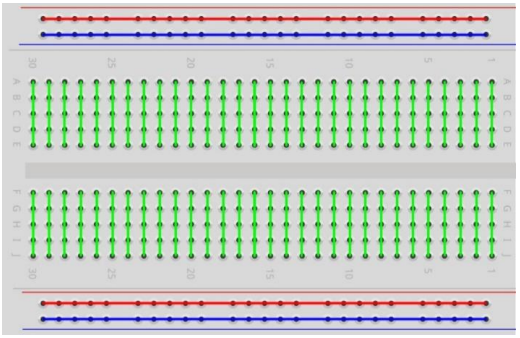
\includegraphics[width=8cm]{../images/board.png}
\caption{Aufbau Entwicklungs-Board \autocite{freenoveTutorial}}\label{Elektrik:DevBoard}
\end{figure}


Für den Aufbau der Schaltung wird ein Breadboard, Abbildung. \ref{Elektrik:DevBoard}, verwendet. Die Verbindungen zwischen den darauf platzierten Bauteilen werden durch Steckbrückenkabel hergestellt, diese werden in das Board gesteckt und durch Klemmung fixiert.
\\

\noindent Die Klemmung wird durch die internen Leiterbahnen erzeugt und ergibt damit eine durchgehende Verbindung wie in Abbildung \ref{Elektrik:DevBoard} durch die farbigen Linien angedeutet wird. 
Dieser Aufbau ermöglicht bis zu fünf direkte Verbindungen innerhalb einer Leiterbahn und insgesamt 60 elektrisch voneinander getrennte Leitungen.
Die äußeren Leiterbahnen sind für die Spannungsversorgung vorgesehen und erstrecken sich über das gesamte Board. Diese Leiterbahnen werden mit \qty{5}{V} bzw. \qty{3,3}{V} betrieben.
Die Verbindungen zwischen dem Micro-Controller und dem Breadboard wird mithilfe eines Extension Boards hergestellt. Das Extension-Board ist so konzipiert, 
dass die einzelnen Pins des Micro-Controllers mit bestimmten Leiterbahnen auf Breadboard verbunden werden.
\\

\noindent Zu beachten ist, dass Insgesamt 40 Leiterbahnen somit nicht frei benutzt werden können, da diese eine direkte Verbindung mit Micro-Controller darstellen.
\begin{figure}[h]
\centering
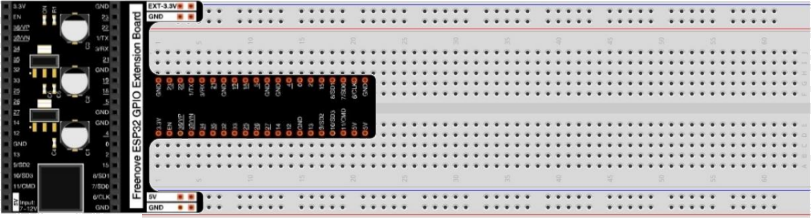
\includegraphics[width=8cm]{../images/ext_board.png}
\caption{Schaltung Entwicklungs-Board \autocite{freenoveTutorial}}
\label{Elektrik:DevBoardext}
\end{figure}

\noindent Die durch die Platzierung des Extensions-Boards verwendeten Leiterbahnen sind für die aktuelle Schaltung unerheblich, da die verfügbaren Leiterbahnen ausreichend sind. Der Vorteil dieser Vorgehensweise besteht darin, dass durch das Stecksystem keine permanente Verbindung erzeugt werden muss. 
Die daraus resultierende Flexibilität ermöglicht ein experimentelles Vorgehen und den Vergleich der potenziell verfügbaren Antriebsarten.

\subsection{Ansteuerung der Motoren}
Für die Umwandlung der elektrischen Signalen des Micro-Controllers in Bewegungen sind zwei verschiedene Motortypen untersucht worden.

\begin{itemize}[h]
	\item Servo-Motor
	\item Gleichstrom-Elektromotor
\end{itemize}

\subsection{Gleichstrom-Elektromotoren}
\noindent Für die Gleichstrom-Elektromotoren werden Motoren aus dem Fischer Technik Sortiment verwendet. 
Diese Motoren sind aufgrund der Produkzugehörigkeit mit den passenden Aufnahmen versehen, um Kompatibilitätsprobleme mit der Mechanik auszuschließen.
\\


\noindent Für die Verwendung innerhalb der Mechanik ist es erforderlich, dass der Motor in beide Richtungen drehen kann und über ausreichendes Drehmoment bei der gegebenen Übersetzung verfügt.
Aufgrund der unterschiedlichen Anforderungen werden zwei unterschiedliche Motoren verwendet.
\begin{itemize}[h]
\item Motor XM \qty{9}{V}
\item Motor XS \qty{9}{V}
\end{itemize}

\noindent Die Leistungsdaten des Motor sind wie folgt definiert. 
\newline \textit{Die Angaben sind bei maximaler Leistung erhoben.}

\begin{table}[h]
  \caption{Leistungsdaten}
  \label{Leistungsdaten}
  \centering
  \begin{tabular}{lllll}
    \toprule
    \textbf{Motor} & \textbf{V} & \textbf{n\textsubscript{max}} & \textbf{I\textsubscript{max}} & \textbf{M\textsubscript{max}} \\
    \midrule
      XM \autocite{motorenXM} & $\qty{9}{V}_{DC}$ & $\qty{337}{U/min}$ & $\qty{0.863}{A}$ & $\qty{0.0587}{Nm}$ \\ 
      XS \autocite{motorenXS} & $\qty{9}{V}_{DC}$ & $\qty{5663}{U/min}$ & $\qty{0.162}{A}$ & $\qty{0.0010}{Nm}$ \\
    \bottomrule
  \end{tabular}
  \end{table}
  
\noindent Da beide Motoren mit jeweils \qty{9}{V} Gleichstrom (DC) betrieben werden, können sie nicht direkt über die Spannungsschiene des Micro-Controllers angesteuert werden, 
da diese maximal \qty{5}{V} liefert. Obwohl ein Betrieb mit \qty{5}{V} möglich wäre, würde dies zu einer Verringerung des Drehmoments führen. Um eine optimale Bewegung zu gewährleisten, 
wird eine \qty{9}{V} Stromversorgung angestrebt. Eine Richtungsänderung der Motoren kann durch das Tauschen der anliegenden Spannung erreicht werden.  

\subsection{Motortreiber}

Für die Ansteuerung der Motoren über den Micro-Controller wird ein separater Motortreiber, L293D, verwendet.
Dieser gehört zur Familie der IC Chips (Integrated Circuit Chip) und beinhaltet zwei interne H Brücken. Dies ermöglicht durch die Verwendung von zwei Kanälen die Drehrichtung 
sowie die Geschwindigkeit des Motors per PWM  zu steuern.

\begin{figure}[h]
  \centering
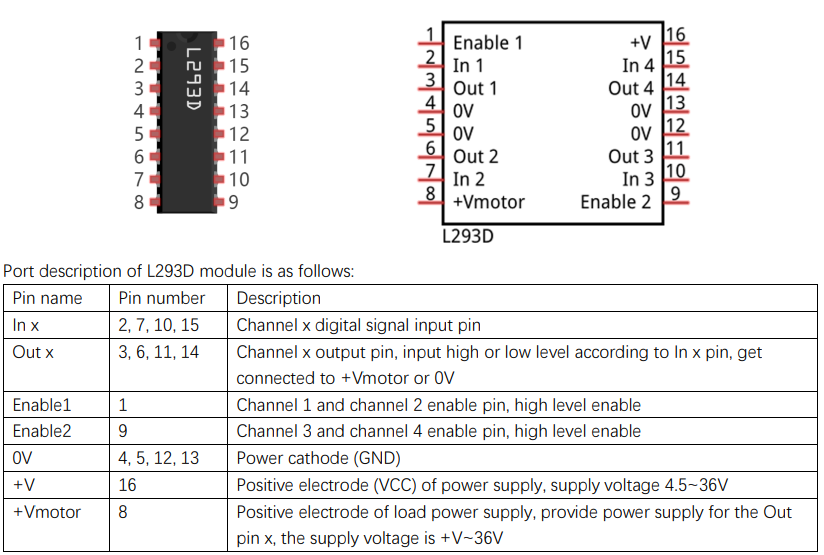
\includegraphics[width=8cm]{../images/L293D.png}
\caption{L293D interner Schaltplan \autocite{freenoveTutorial}}\label{Elektrik:L293D}
\end{figure}

\subsection{PWM}
\emph{PWM} (\emph{Pulsweitenmodulation}) ermöglicht die präzise Steuerung der Drehgeschwindigkeit eines Motors. Dabei wird kein konstantes Signal an den Motor angelegt,
sondern das Signal periodisch zwischen den Zuständen "An" und "Aus" gewechselt. Die Drehgeschwindigkeit wird durch die Anpassung der Pulsweiten innerhalb der Perioden 
bestimmt \autocite{611797}. Aufgrund der hohen Frequenz wird ein konstante Drehbewegung erreicht. 
\\

\noindent Das PWM Signal wird vom ESP32 erzeugt und kann dort entsprechend modelliert werden. 
\\

\noindent In der aktuellen Konfiguration werden jedoch nur zwei Geschwindigkeiten benötigt: Stillstand (0) und maximale Geschwindigkeit. 
Dies wird durch die entsprechende Taktfrequenz in der Software gesteuert und durch die Verbindung der 
spezifizierten Pins des Micro-Controllers mit Pin 2 des Treibers realisiert.
\\

\noindent Die Ansteuerung des Motors über den Treiber wird mithilfe von Pin 1, Pin 2 und Pin 7 realisiert. 
Diese Pins werden mit Digitalsignalen vom Micro-Controller gesteuert.
\begin{itemize}
  \item Pin 1 ist für die generelle Aktivierung des Motors verantwortlich
  \item Pin 2 und Pin 7 steuern die jeweilige Drehrichtung des Motors
\end{itemize}

\begin{table}[h]
  \caption{Ansteuerung des Motortreibers \autocite{l293DataSheet}}
  \label{AnsteuerungMotor}
  \centering
  \begin{tabular}{llll}
    \toprule
    \textbf{Pin1} & \textbf{Pin2} & \textbf{Pin7} & \textbf{Motor Bewegung}  \\ 
    \midrule
    H             & H             & L             & Drehung im Uhrzeigersinn        \\
    H             & L             & H             & Drehung gegen den Uhrzeigersinn \\
    L             & X             & X             & Keine Drehung                   \\ 
    \bottomrule
  \end{tabular}
  \end{table}
  
\noindent Tabelle \ref{AnsteuerungMotor} zeigt die Kombinationen der Zustände von Pin 1, Pin 2 und Pin 7 und die resultierende Motorbewegung:

\noindent Hierbei steht \grqq{H}\grqq{} für den High-Zustand (1) und \grqq{L}\grqq{} für den Low-Zustand (0). Wenn Pin 1 auf Low (L) gesetzt wird, wird der Motor nicht gedreht.

\subsection{Achsenansteuerung}

Aufgrund der höheren Gewichtslast und der Sicherstellung einer konstanten Geschwindigkeit, wird die $x$-Achse durch eine XM Motor betrieben.
Für die $y$ und $z$-Achsen kann die schwächere XS Variante des Motors verwendet werden.

Alle Motoren benötigen unabhängig deren Leistungsdaten einen eigenen Treiber, damit jeder Motor in beide Richtungen angesteuert werden können.

\subsection{Servo-Motor}

Als Alternative könnte ein Servo-Motor verwendet werden, der die Höhe der $z$-Achse über einen Arm verändert. 
In diesem Fall könnte auf den Treiber verzichtet werden. Allerdings wäre die Systemkompatibilität mit der Mechanik aufgrund der Nicht-Fischertechnik-Teile nicht gegeben. 
Daher wurde trotz des zusätzlichen Treibers ein Fischertechnik DC Motor für die $z$-Achse verwendet.

\subsection{Schaltplan}
\begin{figure}[h]
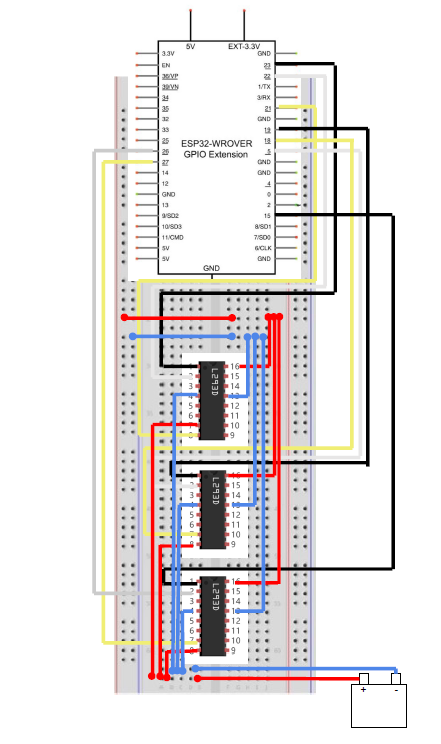
\includegraphics[width=8cm]{../images/schaltplan.png}
\caption{schematische Darstellung der Verbindung zwischen den Treibern und des Micro-Controllers}\label{Elektrik:Schaltplan}
\end{figure}

Aufgrund der aufgeführten Anforderungen und Eigenschaft, ergibt sich, wie in Abbildung\ref{Elektrik:Schaltplan}, folgender elektrischer Aufbau auf Basis des ESP32-WROVER-Boards.
\subsection{IO Eingabe}

Für die Kommunikation mit dem Benutzer wird ein 4x4 Martix Keypad verwendet. Die Verbindung zwischen Keypad und Micro-Conntrollers wird über das Breadboard hergestellt. 
Die nötigen 8 Pins werden in den entsprechenden Leiterbahn des Breadboard gesteckt und werden durch das Extension Board  direkt auf den Pin des Micro-Controllers verbunden.

\begin{figure}[h]
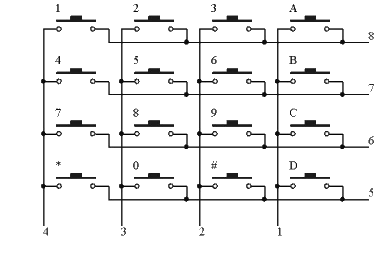
\includegraphics[width=8cm]{../images/keypad.png}
\caption{Aufbau des Keypad \autocite{freenoveTutorial}}\label{Elektrik:Keypad}
\end{figure}

Wie in Abbildung \ref{Elektrik:Keypad} zu sehen ist, ist das Keypad mit jeweils 4 Spalten und Zeilen aufgebaut. Diese sind entsprechend mit dem jeweiligen Tasten als Schalter verbunden. 
Sobald eine Taste betätigt wird, wird ein entsprechender Schaltkreis geschlossen und die jeweilige Taste kann bestimmt werden.

Die Tasten 1 bis 9 repräsentieren entsprechend die Felder des Tik-Tak-Toe Spielfeldes und dienen zur Auswahl des gewünschten Feldes. 
Die weiteren Tasten werden zur Steuerung der einzelnen Achse verwendet.
Dies ermöglicht zum einen einen Test der Achse, zum anderen kann somit die Startpostion für das Spiel Manuel justiert werden.

Durch die Verwendung des Keypad konnte die gesamte Interaktion für die Bedienung des Roboter auf diese Schnittstelle abgebildet werden.

\section{Software}

\subsection{Steuerung}
Für die Steuerung des Roboter standen verschiedene Methoden zur Verfügung. Die einzige Anforderung dabei
war es, dass die Steuerung in der Lage ist, die einzelnen Motoren und weitere Hardware Komponenten
zu kontrollieren. Hierzu haben wir uns folgende Möglichkeiten überlegt:

\begin{itemize}
  \item Steuerung über einen externen Computer
  \item Steuerung über eine mobile App
  \item Steuerung über einen Prozessor mit integriertem Code
\end{itemize}

Die Steuerung über einen externen Computer wurde als erste Lösung betrachtet. Der Vorteil
ist hier, dass man auch eine vollfunktionsfähigens Betriebssystem mitsamt allen dafür existierenden
Paketen und Programmiersprachen zurückgreifen kann. Da aber das vollständige Betriebssystem auch
dazuführt, dass Services gestartet werden, die mit der eigentlichen Aufgabe des Roboters nichts zu
tun haben, wurde sich gegen diesen Ansatz entschieden. Zusätzlich erzwingt eine solche Steuerung
eine dauerhafte Verbindung zu dem Computer. Dies ist nicht erwünschens wert, da der Roboter autonom
handlungsfähig sein soll.

Als zweite Wahl kam die Steuerung über eine mobile App ins Spiel. Dies ermöglicht es, dass die
eigentlichen Bewegungen auf einem Gerät mit viel Prozessorstärke ausgeführt werden kann und dann nur
noch an den Roboter übermittelt werden muss. Somit ist auch der Zweck des Roboters
durch die Veränderung des Programmcodes auf dem Smartphone anpassbar. Die Schwachstelle hier ist,
dass weiterhin ein eingebetteter Prozess in Roboter vorhanden sein muss, der eine stabile
Kommunikation mit dem Mobilegerät besitzen muss. Während des Bau unseres Prototypen ist es den Autoren,
nicht gelungen eine stabile Kommunikation per Bluetooth mit einem iOS Gerät herzustellen.
Was die Nutzung des Roboters weiter einschränkt. Kommunikation per Wifi konnte hergestellt werden,
allerdings müssen sich sowohl das Mobiltelefon als auch der Roboter im 
selben Netzwerk befinden. Dies setzt eine Eingabemöglichkeit auf dem Roboter voraus oder dass
die Zugangsdaten vordefiniert sind. Beide Möglichkeiten sind in diesem Projekt nicht realisierbar,
da die Motorsteuerung schon alle Pins belegt und der während der Entwicklung und dem Einsatz in der
Hochschule in unterschiedlichen Netzwerken laufen können soll.

Letzlich fiel die Entscheidung darauf allen Code auf dem eingebetteten Chip zu spielen und dort
das gesamte Spiel zu implementieren. Dies bringt auch den Vorteil, dass der Roboter mit der Verbindung
zum Strom sofort spielbar ist. Außerdem werden so alle Fehlerfälle ausgeschlossen, die durch die
drahtlose Kommunikation zustande kommen könnten. Nachteilig ist hier, dass der Programmcode nur
vergleichsweise umständlich verändert werden kann. Da der Roboter nur für den aktuell singulären
Zweck des Tik-Tak-Toe spielen geschaffen wurde, wiegt dieser Nachteil allerdings nicht schwer.

\subsection{Tik-Tak-Toe-Algorithmus}

Für den Tik-Tak-Toe Algorithmus wurde ein in C implementierter Algorithmus erstellt, der direkt auf
den ESP32-WROOM eingebettet wurde. Hierbei wurde großer Wert auf eine kompakte und einfache
Implementierung gelegt, da der gesamte Programmcode einschließlich des während der Laufzeit
gehaltenen Speichers in die 520KB Speicher des Chips passen mussten.

Um den Code einfach zu halten, wurde die Spielausführung auf einen der beiden CPU Kerne beschränkt.
Damit ist die Logik des Spiels einfach nachzuvollziehen, da sie von oben nach unten gelesen werden kann.
Um dieses Ziel zu erfüllen, wurden alle Bewegungen des Roboters als blockierende Calls im Programm
umgesetzt.

Kompakt wurde die Speichernutzung gehalten, indem das Spielfeld in zwei einzelne 16\,Bit Integer integriert wurde.
Da das Spielfeld nur 9 Felder hat, werden nur 9\,Bit pro Spieler benötigt, um zu speichern, ob der Spieler
auf dem jeweiligen Feld aktiv ist. Damit sind 16\,Bit Integer die kleinst mögliche Speichereinheit, in der
diese Daten für einen Spieler gespeichert werden kann. Alle möglichen Gewinnstellungen werden entsprechend
auch von einem einzelnen 16\,Bit Integer repräsentiert. Um herauszufinden, ob ein Spieler gewonnen hat, kann
nun die Gewinnposition per bitweisem UND mit dem Spielfeld vergleichen und wenn das Ergebnis der Operation
der Gewinnposition entspricht, hat der Spieler diese erreicht.

Bei einem Spiel zwischen Mensch und Maschine nutzt der Roboter die enthaltenen Gewinnpositionen als
Entscheidungsgrundlage für den nächsten Zug. Dabei wird geprüft, welche der Gewinnpositionen noch erreichbar
sind. Danach wird ermittelt, wie viele Züge dazu noch zu ziehen sind. Die Gewinnposition mit den
wenigsten Zügen wird versucht zu erreichen. Falls mehrere Gewinnpositionen gleich gut gewichtet wurden
oder noch kein Zug gespielt wurde, wird zufällig eine Zielposition ausgewählt. Die Berechnung läuft
dabei nach jedem Zug, wodurch der Roboter auf den Zug seines Gegners reagieren kann.

\subsection{Abstraktion Hardware und Software}

Um den Autoren die Möglichkeit zu geben, zu unterschiedlichen Zeitpunkten an dem Roboter arbeiten
zu können, wurde die Software und die Hardwareentwicklung per Abstraktionsstufe getrennt. Hierbei wurde
ein mindestmaß an Funktionalitäten definiert, die der Roboter bereitstellen können muss, um Tik-Tak-Toe
ausführen zu können. Diese Funktionalität wurde dann als Schnittstelle zwischen der Hardware und Software
genutzt. Damit wurde eine unabhängige Entwicklung der Softwarefunktionalität von der Hardware geschaffen.

Die Hardware Funktionen haben hierbei keinerlei Wissen und Verantwortung über den aktuellen Spielstand.
Wählt ein Spieler einen Zug aus, der nicht mehr spielbar ist, so erkennt die Spielelogik das und führt
entsprechend die entsprechende Bewebungsfunktion aus, um dies zu kommunizieren. Dies sorgt für eine
optimale Abstraktion und Testbarkeit der Software.

Die Schnittstelle lässt sich in 4 Teile unterteilen.

\begin{minted}{c}
void waitUntilGameStarts();
int getFieldSelectedByPlayer();
\end{minted}

Der oben aufgeführten erste Teil beinhaltet Funktionen, deren Aufgabe alle Nutzereingaben abdecken.
Ihre Aufgabe ist es so lange die weitere Ausführung des Programms zu blockieren,
bis ein Spiel gestartet werden kann oder bis der Nutzer ein Feld gewählt hat.

Beide Funktionen bauen dabei auf der Tastatur auf. Ein Spieler zeigt an, dass er ein Spiel starten
möchte, indem er die Taste \enquote{1} für ein Spiel gegen den Roboter oder die Taste \enquote{2}
für ein Spiel zwischen zwei Menschen auswählt. Zur Selektion eines Spielzuges stellt die Tastatur
das Spielfeld dar. Dabei entspricht jede nummerische Taste einem Feld im Spielfeld. So kann
gewählt werden, welcher Spielzug der Spieler als nächstes spielen möchte.

In diesen Funktionen wurden später auch die Möglichkeit eingebaut, alle Achsen des Roboters von 
Hand zu steuern, um ihn richtig ausrichten zu können. Dies ermöglicht es, dass hardware-nahe Funktionen
nicht im Spielalgorithmus verankert werden müssen und dennoch gut eingebaut werden konnten.

\begin{minted}{c}
void moveRobotArmToOrigin();
void moveRobotArmToFieldOne();
void moveRobotArmToFieldTwo();
void moveRobotArmToFieldThree();
void moveRobotArmToFieldFour();
void moveRobotArmToFieldFive();
void moveRobotArmToFieldSix();
void moveRobotArmToFieldSeven();
void moveRobotArmToFieldEight();
void moveRobotArmToFieldNine();
\end{minted}

Im aufgeführten zweiten Teil, sind alle Funktionen beinhaltet, die Bewegungen des Roboter darstellen. Diese haben
zum einen den Zweck zu einem bestimmten Spielfeld und wieder zurück zu kommen. Zu beachten ist hier,
dass die Hardware den aktuellen Ort des Stiftes kennen muss, um diesen nach dem entsprechenden Funktionsaufruf
wieder zurück zum Ausgangspunkt navigieren zu können.

Zur Navigation des Robots wird auf allen Achsen auf Zeitangaben gesetzt, in denen die Motoren aktiviert werden. Die
aktuelle Position des Roboters wird aus der Zeit der aktivierten Motoren abgeleitet. Die zugrundeliegende Annahme
ist, dass sich ein Motor in beide Richtungen gleich schnell dreht. Die Größe des impliziten Koordinatensystems wird
daher durch die Größe des Spielfelds festgesetzt.

Dies ist der dritte Teil:

\begin{minted}{c}
void drawCross();
void drawCircle();
void drawHorizontalWinningLine();
void drawVerticalWinningLine();
void drawTopToBottomWinningLine();
void drawBottomToTopWinningLine();
\end{minted}

Der dritte Teil der Schnittstelle beschäftigt sich mit den Zeichenanweisungen des Roboters. Hierbei legt der
Tik-Tak-Toe Algorithmus fest, was gezeichnet werden soll. Die exakten Details der Bewegung und wann der Stift
auf das Blatt abgesetzt und gehoben werden muss, wurden auch hier als hardware-spezifisch deklariert.

Der Roboter zeichnet ein Kreuz, wie in Tik-Tak-Toe üblich, ersetzt aber den Kreis durch ein Viereck. Dies ist
der einfacheren Ansteuerung der Motoren bei geraden Linie geschuldet. Um einen Kreis zu zeichen, muss die
Geschwindigkeit des Motors sowohl auf $x$ als auch auf $y$-Achse in kurzen Intervallen angepasst werden. Einen 
guten Kreis zu erhalten wurde hierbei als zu aufwändig eingestuft und der Fokus eher auf das Spielverhalten
des Roboters gelegt wurde.

\begin{minted}{c}
void showCannotPlayMove();
\end{minted}

Zu letzt benötigt der Roboter eine Möglichkeit zu kommunizieren, dass ein Spielzug nicht gespielt werden kann,
weil dieser schon von einem anderen Spieler zuvor gespielt wurde. Dies stellt den vierten und letzten Teil der
Schnittstelle dar.

Die Aufteilung der Schnittstelle ermöglicht dabei nicht nur die getrennte Entwicklung von Hardware und Software,
sondern auch, dass die Software extern und automatisiert getestet werden konnte. Damit wurde die Funktionalität des Algorithmus
sichergestellt und erlaubte eine Test-basierte-Entwicklung auf einem leistungsstarken Computer ohne direkten
Hardwarezugriff zu benötigen.

\section{Fazit und Ausblick}

\subsection{Offene Probleme}

Auf mechanischer Ebene besitzt der Roboter viel Spiel, was die exakte Steuerung schwierig macht. Ein Problem mit der Anordnung
des Motors und des kleinen Zahnrades ist, dass die
Antriebswelle nicht fixiert werden kann und sich erstmal schräg stellt, bevor das große Zahnrad anfängt sich zu drehen. Jegliche
Idee die Welle zu fixieren hätte dazu geführt, dass die Konstruktion an der Kette reibt. Um dieses Problem zu lösen hätte es größere
Umbauten am gesamten Plotter benötigt, die aufgrund des späten Zeitpunktes, zu dem der Motor angekommen ist, nicht mehr möglich waren.

Auch die Stabilität anderer Bausteine verursachen Spiel im Roboter. So sorgt das Aufsetzen des Stiftes dafür, dass dessen Halterung
leicht vom Papier weggedrückt wird. Dies ist nötig, da der Stift mit etwas Druck auf dem Papier aufgesetzt werden muss, um
Tinte zu hinterlassen. Zwar konnte der benötigte Druck durch Einsatz eines Filsstifts statt eines Kugelschreibers reduziert werden,
allerdings wird weiterhin etwas Druck benötigt, was die Halterung anhebt.

Ein ähnliches Problem besitzt auch die $y$-Achse welche sich leicht zusammenzieht, wenn der Schlitten an das Ende der Achse ankommt.

Einen zusätzlichen Verbesserungspunkt stellen die Motoren dar, da sie nicht in beide Richtungen exakt gleich schnell drehen. Eine
mögliche Lösung sind hier Endschalter, die aktiviert werden, sobald der Roboter das Ende der jeweiligen Achse erreicht. Diese wurden
auf Grund an mangelnder Anzahl an Pins am Chip und späten Auftretens im Projekt nicht genutzt.

\subsection{Positive Aspekte}

Als ein positiver Aspekt stellte sich der verwendete ESP32-WROOM heraus. Der Chip erlaubt dem Roboter nicht nur ohne externe Steuerung
auszukommen, sondern bietet mehr Leistung als der Roboter benötigt. Ein Großteil des Spiels besteht aus Warten auf die Motoren und die
Spiellogik ist nicht sehr leistungshungrig, sodass noch mehr Funktionlitäten mit dem Roboter abgebildete werden könnten.

Auch die Nutzung von Fischertechnik brachte sehr viele Vorteile. So konnte sehr schnell über die Mechanik des Roboters iteriert werden,
was eine hohe Entwicklungsgeschwindigkeit ermöglichte. Zusätzlich dazu erlaubte das Steckkastensystem das Erkunden neuer Lösungsmöglichkeiten
inklusive einfacher Rückbauten im Falle eines nachteiligen Ergebnis. Auch die Kombination aus Plastik und Metal führt zu einer einfachen 
Anpassbarkeit mit gleichzeitig robustem Unterbau, um das Gewicht des Roboters optimal zu tragen. Nichtsdestotrotz lässt sich ein Teil des
Spiels auf die Bauteile zurückführen. Im gesamten Blick haben die Vorteile der schnellen Veränderung im Projekt allerdings überwogen.

Als letzten positiven Aspekt ist die Abstraktion der Software und Hardware zu nennen. Dies ermöglichte einen testbasierten
Entwicklungsansatz, der keinen ESP32-WROOM voraussetzte, um ausgeführt zu werden. Zwar hatten alle Teammitglieder Zugriff auf entsprechende
Chips, aber diese hätten immer eine langsames Aufspielen vorausgesetzt, was die Entwicklung verlangsamt hätte. Auch konnten so mehrere
Teammitglieder parallel und unabhängig von einander sowohl an der Software als auch an der Hardware iterieren. Gleichzeitig war die
Integration der beiden Systeme sehr einfach möglich und kann daher nur empfohlen werden.

\subsection{Ausblick}

Der aktuelle Roboter ist eine gute Grundlage für alle Arten an Aktivitäten, die etwas mit Zeichnen zu tun haben. Wenn die Präzision
gesteigert werden kann, können auch Spiele implementiert werden, die mit kleineren Feldern auskommen müssen. Die könnte beispielsweise
4-Gewinnt ermöglichen.

Auch der generellen Verwendung des Roboters als Plotter steht nichts im Weg. Zwar sind aktuell nur gerade Linien implementiert, aber
auch Kurven können mit der aktuellen Motorensteuerung umgesetzt werden, was dem Roboter ermöglicht beliebige Bilder zu zeichnen.

% Literaturverzeichnis
\addcontentsline{toc}{section}{Literatur}
\printbibliography

\end{document}
